\section{Recognition and pose estimation pipeline} \label{sec:linemod-pipeline}

In this chapter a pipeline similar to the one introduced in
\cite{linemod-pipeline} is presented, which is used to detect and estimate
the pose of the objects to be recognized. First a template matching approach is
used to detect the objects, then matches are progressively excluded (false
positives detection) based on hue values; finally valid matches are
progressively refined by physically moving a precision depth camera and
performing depth-based alignment of the match and the real object.

\subsection{Image matching using the Line-MOD algorithm} \label{sec:match-with-linemod}
The proposed object recognition algorithm is started by an upper
algorithm, managing the whole gripping strategy, which requires to the
recognition system to find a set of known objects into an RGBD
image. Three images are actually passed for recognition, which are
assumed to be registered at a pixel level: the RGB image of the scene,
the corresponding depth image, and a mask. The latter is an 8-bit
image with the same size of the whole scene, having each pixel with
value 255 if the pixel must be evaluated for recognition, and 1 if it
must be discarded.

For each object, the recognition system can be instructed to use a
recognition algorithm different from Line-MOD: if it isn't, the object
is assumed to correspond to a valid object for the Line-MOD
training database. This is the case which is treated in the rest of
this section.

For each model which has to be recognized using Line-MOD, the
corresponding training database is read from memory; this database
is created at initialization time from a directory tree which
associates each object's ID with the corresponding detector
description (number of modalities, type of modalities, mesh used for
rendering the object, etc.) and with the list of templates which are
associated to the object. After reading the objects, all of their
templates are merged together to form a single template list which
will be used for matching: information about the nature of each
template is mantained inside the template itself, as each item of the
list contains both the template's features and some metadata, like the
object ID the template refers to, the pose of the object which
corresponds to it, and additional informations which can were saved
during training (for example, if a simple filtering algorithm for false
positives  based on RGB histograms has to be implemented, it is enough
to link these data to the templates when training, and they will be
easily recovered when matching); the features of the image which is
included into the input mask are then computed, their binary
representation and response map are generated as described in
sec.~\ref{sec:linemod-binary}, and each template is matched upon
this. As the most intensive part for Line-MOD is the computation of
the reponse map for the scene's image, while template matching is
almost istantaneous, it is very convenient to match all the possible
templates in a single pass, as this will require the scene image to be
processed only once.

For each match, a corresponding matching percentage is defined. Given
the similarity function of eqn.~\ref{eqn:similarity-function}, the
percentage $S_\%$ of match for each template $T$ can be easily defining by noting
that the maximum possible similarity score, given when the two
images match perfectly, is given by the similarity function of the
scene's section $I$ with itself:

\begin{equation} \label{eqn:match-percentage}
  S_\%(T) = \frac{S(I,T)}{S_{max}(I)} = \frac{S(I,T)}{\sum_{p \in I}
    \left( \tau I_{p} \right)}
\end{equation}

In order to avoid considering matches which bring too little
information due to the extremely low matching area, a filter is put on
all the matches that come out from this cycle, checking both the
matching percentage defined in eqn.~\ref{match-percentage} to be over
a threshold $t_\%$ and the total area (in pixels) of the template
which matched to be over a threshold $t_{\text{area}}$. All the
matches that pass this check are kept as valid and stored into a
match list.

When this loop exits, thus, it will output a list of matches which are
tolerably strong and matched with a valid object pose and ID.

As it operates on multiple objects at the same time, this algorithm
will make sure to find at least a valid match for each object before
exiting; if this does not happen at the first iteration, the
Line-MOD algorithm is started again, and the minimum similarity
threshold $t_\%$ is decreased by a factor 0.95; matches (which can
uniquely identified by the object ID, template ID, and matching
coordinates $(u,v)$) which have already been processed will be
discarded in the following loops in order not to count them twice.

\subsection{Pyramidal matching for faster match}
As with most of the vision algorithms operating on medium-sized (VGA)
to large-sized  images, it is often unconvenient to process the
whole source image each time a detection query is made from a part of
the program. The solution used in this cases to significantly speed up
the performance of the recognition pipeline is the usage of
\emph{image pyramids}.

If pyramids are used to process a sample, the recognition algorithm
doesn't actually process the whole if it: instead, before recognition
a set of derivative images are built from the source one, each of a
smaller scale (usually, halved scale), until a predefined scaling
level is reached. In order not to lose too much information,
especially regarding image's features -- which, by definition, often
are present only in a narrow range of the image -- scaling
is not done roughly by downsampling the image: instead, first the
full-scale image is blurred using either a \emph{gaussian} or
\emph{laplacian} transform, and downsampling is done only after this
step. The images' set (the pyramid) is built top-down, iterating over
the lowest-scale image to produces the subsequent one; the mathematics
behind this transformations has been well studied in literature and is
omitted here, a good explanation for it can be found in most computer
vision books such as \cite{computervision}. An example of the pyramidal
images' building process is seen in fig.~\ref{fig:pyramidal-images}.

\begin{figure}[htbp]
\centering
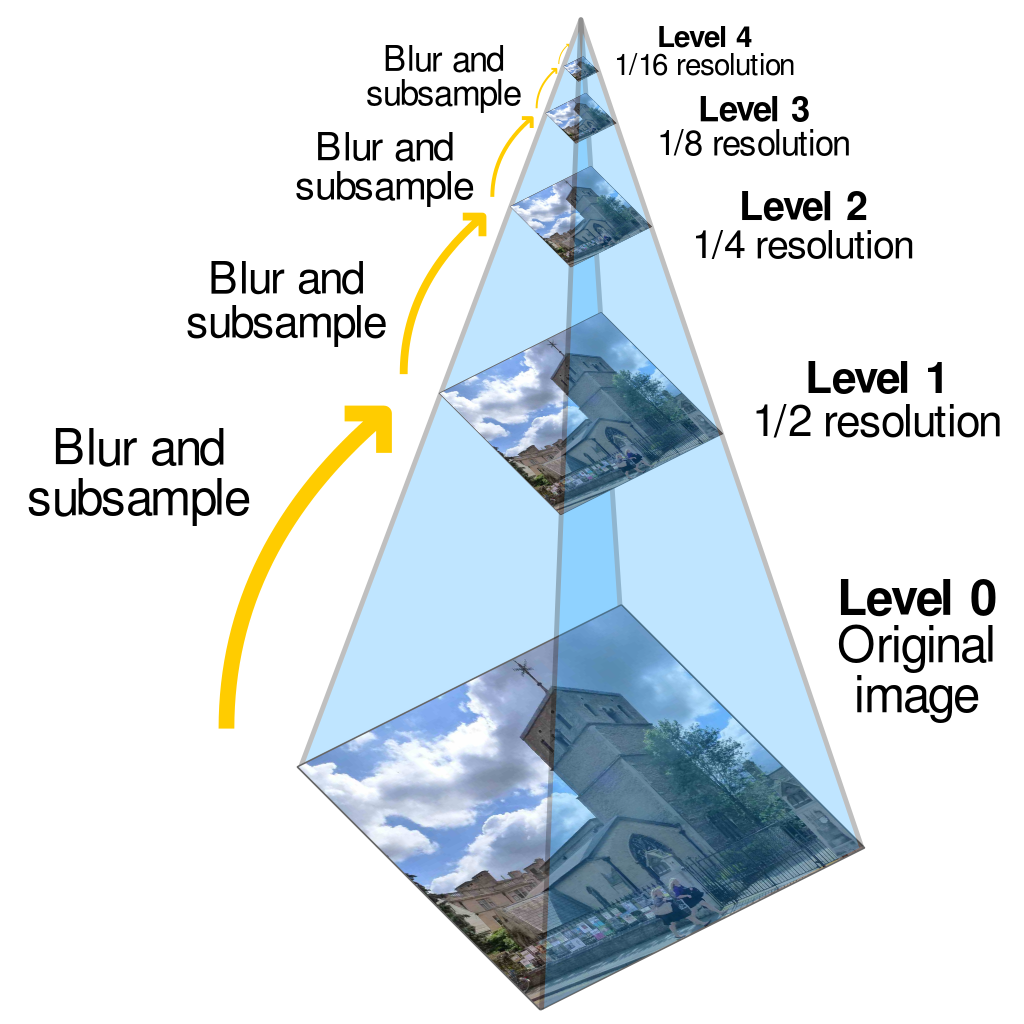
\includegraphics[width=3in]{./Graphics/pyramidal-images}
\caption{Building an image pyramid from an image: at each iteration,
  the top level of the pyramid (i.e. the image with the smallest
  scale) is blurred and downsampled to produce the next pyramidal
  level. Image source: Cmglee (own work) (Cc-BY-SA 3.0)
  \label{fig:pyramidal-images}}
\end{figure}

The Line-MOD algorithm's implementation used into this project, based
on the one implemented into the OpenCV libraries, actively uses
pyramidal matching in order to speed up its operation. When an
object's model is requested to create and store a Line-MOD template
for subsequent usage, it takes the input images and creates a
two-levels pyramid from them. It then extracts features and template
data for both levels; in this sense, a template for this detector type
is actually a set of templates, each operating at a different
scale. When the detector is told to use its informations to
match templates over an image, filtering matches with a certain
confidentiality threshold $t$, it first builds the same pyramid from
the source image, and searches for template matches on it. Templates
are accepted only if they match within a certain threshold, which is
set to a fraction of $t$ in order to sustain the loss of information
that the lower scaling factor brings with it. Although the matching
threshold is lowered at this step, this already helps a lot in
discarding templates which are not present into the source image, and
thus fastens the operation, as matching at each subsequent pyramidal
level means having one order of magnitude less of complexity in
matching.\footnote{although matching templates is an almost
  instantaneous operation, the big number of templates which have to
  be matched into the image has to be considered}. Only the templates
which survive this first matching step are matched against the
full-scale image; also, as matching at a deeper level already gives a
good hint about where each template could be present into the whole
image, when matching at full scale only those parts which are within a
small radius with respect to the previous match's origin have to  be
searched, which brings to further performance improvement on the algorithm.

The important thing to notice about all of this process is that,
starting from full-scale images (when recognizing) and templates (when
training) the whole process is \emph{totally transparent} to the user:
this is an obvious advantage as the user probabily will not be willing
to further manipulate its source images when matching if not strictly needed.

\subsection{False positive rejection based on hue values}
The first step of pose matching is made by purpose to be overly tolerant in
template matching. This is because the used objects are quite small and simple
in shape - which can reduce the number of features to match - and at the first
step are seen from far away ( more than 1 meter ) in order to maximize the
field of view without increasing the needed number of cameras. The counterpart
for being sure to match \emph{at least} something is having a huge number of
  false positives, which must be recognized and excluded before starting the
  alignment.


To do this, after performing each match together with a rough pose estimation,
the object is rendered again into its estimated position, and the portion of
source image corresponding to the render is taken. The two images are then
compared on a per-pixel basis, considering only the pixels that lie on the
depth mask created during rendering. 

Before comparing, the two images are converted to the HSV colour space, and
comparation is done based on the hue values. This allows to only consider the
actual colour of the model and match, and discard all information about
surface behaviour with respect to light, together with variations in the images
depending on different lightning conditions.

HSV colour space has singularities on the hue dimension when the chosen pixel is
either black or white; in this case, in effect, the hue of the pixel is
undefined due to the low saturation or low luminosity (\emph{value}). To fix
this, white and black pixels are turned to be zero-saturated, zero-valued
pixels with fixed hue, corresponding to yellow (for white) and blue (for
black). When matching, these are treated as special values and two pixels are
said to match either if their actual hue match (which
is robust to moderate lightning changes) or if their modified hue, saturation
and values match
(which happes if both the model and the scene appear to be actually white or
black). 

After computing the new HSV values, the four resulting images (two belonging to
the source image, two belonging to the rendered one) are scaled down of a
factor $K_s$. This makes the four images to be downsampled, and improves the
success rate of the subsequent step as it does minimize small alignment errors
due to the pose estimation error within the template. The render's mask $m$ is
scaled down of the same factor.

After scaling, the mask is first filtered in order to keep only the points for
which the mask's value is 1 (thus correcting the interpolated values on the
border which come out of the scaling algorithm) and then
eroded by a small amount (1 pixel). This allows to further remove the noise
which usually comes into the object's borders.

Finally, for each pixel belonging to the newly created mask, a comparison if
done between the corresponding render's and scene's pixel. If their difference
is below a certain threshold $t$, the two pixels correspond. The corresponding
pixels are counted and the matching ratio $P_{match}$ is computed with respect to the
total number of pixels belonging to the scaled mask:

\begin{equation}
P_{match}=\frac{\text{count}\left[(u,v) : m_{u,v}=1 \wedge \left( \lvert
\text{Hue}(r_{u,v})-\text{Hue}(s_{u,v})\rvert < t \vee R_{u,v}=S_{u,v} \right)
\right]
}{\text{count}\left[ (u,v) : m_{u,v}=1 \right] }
\end{equation}

Here, $r$ indicates the scaled-down render, $s$ indicates the scaled-down scene
portion, while $R$ and $S$ indicate the corresponding images with modified hues.

The whole matching and filtering part is repeated until at least one match
passes the filtering step. If no valid matches are found during the first
iteration, the threshold level for the LineMOD algorithm is decreased
just like it was done in the previous step of the pipeline; in this
way, objects with small, partial occlusions can be recognized.

If the threshold $t_\%$ falls below a threshold $t_{\%,\text{bad}}$
and no valid matches have still been found to pass this check for every object, however, the
algorithm exits anyway: exeperimental tests have, in fact, shown that
when the matching threshold becomes below about $80\%$ the algorithm
thends to recognize almost every template as matching, but it will
still fail to recognize correctly the object in its correct
position. This will lead to a huge number of false positives (about
$50\%$) of the total templates, and the hue matching step described in
this section will in turn last several minutes just to continue
failing, which is a situation to avoid. 

\subsection{Point cloud alignments and pose refinement}
The matches that passed the first false-positive rejection step are saved and
sorted based onto their matching percentage. At this point, matches are probably
valid, but only colour information has been considered. Also, a good pose
approximation has been obtained for each match, but coming from a template, it
is not precise enough to be used for grasping. To overcome these problems,
another step is required for each match, which is pose refinement through point
clouds' alignment. In this step, colour information is dropped, and only depth
information is used. 

The Microsoft Kinect RGBD camera provides good depth informations for the template-matching
requirements, but it is not suitable for precisely find the pose of an object
for grasping. This is due mainly to the limitations of its depth sensor, having
a nonlinear depth error of about $1\%$\footnote{TODO:link at MS device page}.
Although this is quite a standard error, it must be combined with the minimum
depth range of $80\unit{cm}$ for the sensor. This leads to an error of about
$1\unit{cm}$ on the depth's values. Also, the field of view of the (fixed)
kinect does not allow to precisely detect the object's pose, as the depth error
increases the more the obejct is not centered with respect to the sensor. As a
higher precision is needed for good 
object grasping, a dedicated, precision depth sensor (\emph{Structure Sensor by
Occipital})has been mounted onto the robot's arm.


This camera's specifications\footnote{http://structure.io/developers} are much better than the kinect's ones, although it
does not provide RGBD images but only depth informations -- hence the need for two
different cameras; it has a much lower minimum range of $40\unit{cm}$ and is suitable for
precision depth measurements, having a maximum error of about $1\%$, which comes
down to $0.15\%$ at $40\unit{cm}$ of distance. This means having an absolute
error of less than $0.2\unit{mm}$ when the camera is close enough to the object.

As the matches already provided a good estimation of the object's position, the
iterative closest point algorithm explained into sec. \ref{sec:icp} can be
applied. 

First, the point cloud for the scene is obtained as explained in sec. \ref{sec:cloud-reconstruction}.
As explained, a scene's snapshot obtained by the precision depth
sensor used and the alignement process is done upon it. In order to
do this, the found match is rendered again into the position in which
it would be as seen from the camera -- whose extrinsic caractheristics
are known because of the fixed locations of the bin; if this was not
the case, it would be enough to find it again at before rendering
using the algorithms of sec.~\ref{sec:camera_calibration}, as they
have neglibible cost with respect to the whole recognition pipeline.
As the mask of the render has already been computed, it is exploited at this
point and only the part of the scene corresponding to the actual
object, increased by a low margin, is
transformed to a 3D point cloud.

During the process of 3D reconstruction a lot of invalid values can be
generated: these are the points for which the depth sensor failed to obtain a
valid measurement, and are ignored from this same algorithm. Two kinds
of values are dropped: those for which the depth measurement is
outside the range specified into the camera's specifications, which
is increased by a small margin to keep uncertainties into account, and
those for which the camera actually reports a $NaN$ value (e.g. in
case of a reflecting surface, for which the speckles patterns results
too heavily distorted).

Both the model's and the scene's cloud are moved to be in global
coordinates after reconstruction; this is done by transforming them
with the inverse of each extrinsic transformation.

When this is done, it will be very probable that the two clouds will
have different point densities, especially for the process of
information dropping coming from the recognition pipeline. This could
harm the premises of the ICP algorithm, as different point densities
or missing points could cause wrong correspondances between points.

To prevent this situation, after reconstruction and transformation,
both the point clouds are evaluated and filtered through what is
called a \emph{Voxel grid}. This filter creates a 3D grid of fixed
size through all the 3D space occupied by the point cloud, and
maintains the crossings onto the grid which correspond to the cells
occupied by at least one input point. In practice, this means that the
output of a voxel grid having a scattered point cloud as an input is
an approximation of the same point cloud made with \emph{equally
  spaced}, regular points. Using the latter instead of the first for
the ICP algorithm results in benefits to the proper
operation of the algorithm itself, as points' correspondance will
lead to zones of the clouds that actually correspond perfectly into the 3D space.

After tessellating the two point clouds, whose points are set in global
coordinates, the resulting filter outputs are aligned using Iterative Closer Point: if the
algorithm converges correctly, the cumulative transformation
$T_{\text{final}}$ of the ICP is used to transform the initial guess for the object's
  pose and obtain the final, refined pose estimation for the object.

Summing up all the points presented into this chapter, the proposed
system for object detection composes thus a complete system by its
own: in particular, the recognition pipeline is fully automatized and
can, starting from the two images taken from the cameras, arrive to
the estimation of the pose of different objects with sub-millimetric
precision. This system can thus be used with success into the solution
of the stated grasping problem.
